\chapter{Generazione dei Segnali Secondari}\label{segnali_secondari}

%--------------------------------------------------------------------------------------------

Ora si passa a estrarre i segnali mancanti da quelli principali generati al capitolo \ref{segnali_principali}.

%--------------------------------------------------------------------------------------------

\section{Dente di Sega}

%--------------------------------------------------------------------------------------------

Il più facile da generare è sicuramente il dente di sega in quanto tutto quello che serve è un
semplice amplificatore invertente con guadagno pari a uno.

\begin{figure}[H]
    \centering
    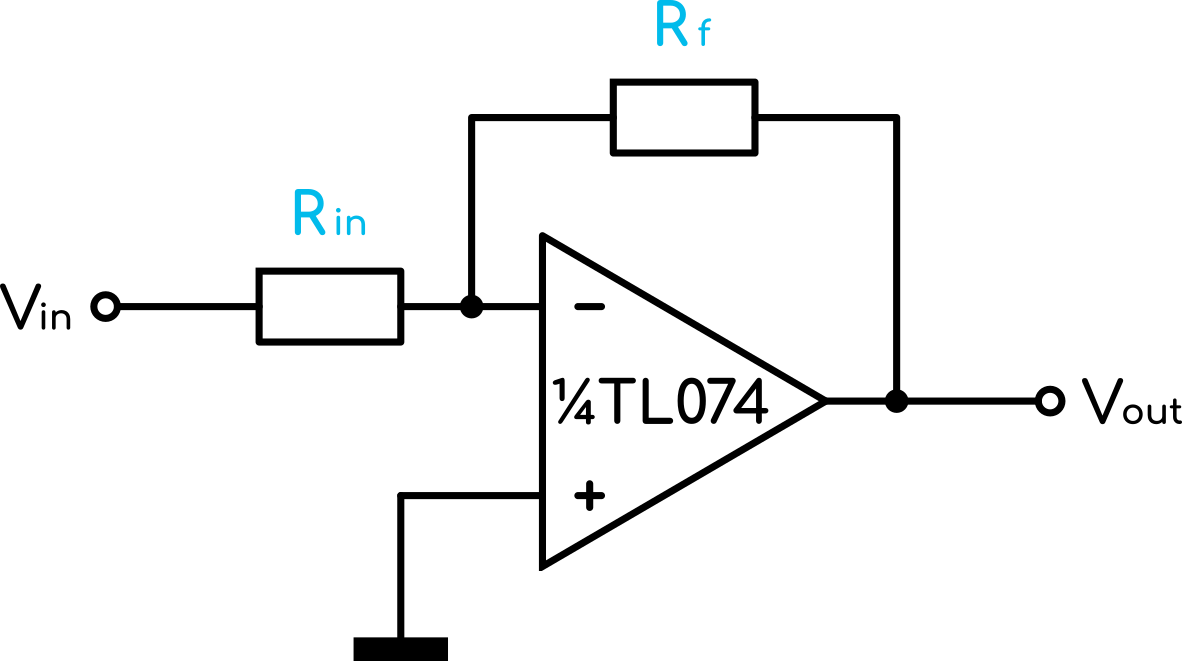
\includegraphics{circuits/inverting_amp_circuit.png}
    \caption{Schema dell'amplificatore invertente}
    \label{inverting_amp_circuit}
\end{figure}

Come sempre l'operazionale utilizzato è un TL074.

Dalla relazione dell'amplificatore invertente vediamo che per avere un guadagno unitario si
deve porre la resistenza di feedback uguale a quella di ingresso, $R_{in}=R_f$.

\begin{equation}
    V_{out}=-V_{in}\frac{R_{in}}{R_f}=-V_{in}\ [V]
\end{equation}

Questo è quanto ottenuto in uscita:

\begin{figure}[H]
    \centering

    \begin{subfigure}{.5\textwidth}
        \centering
        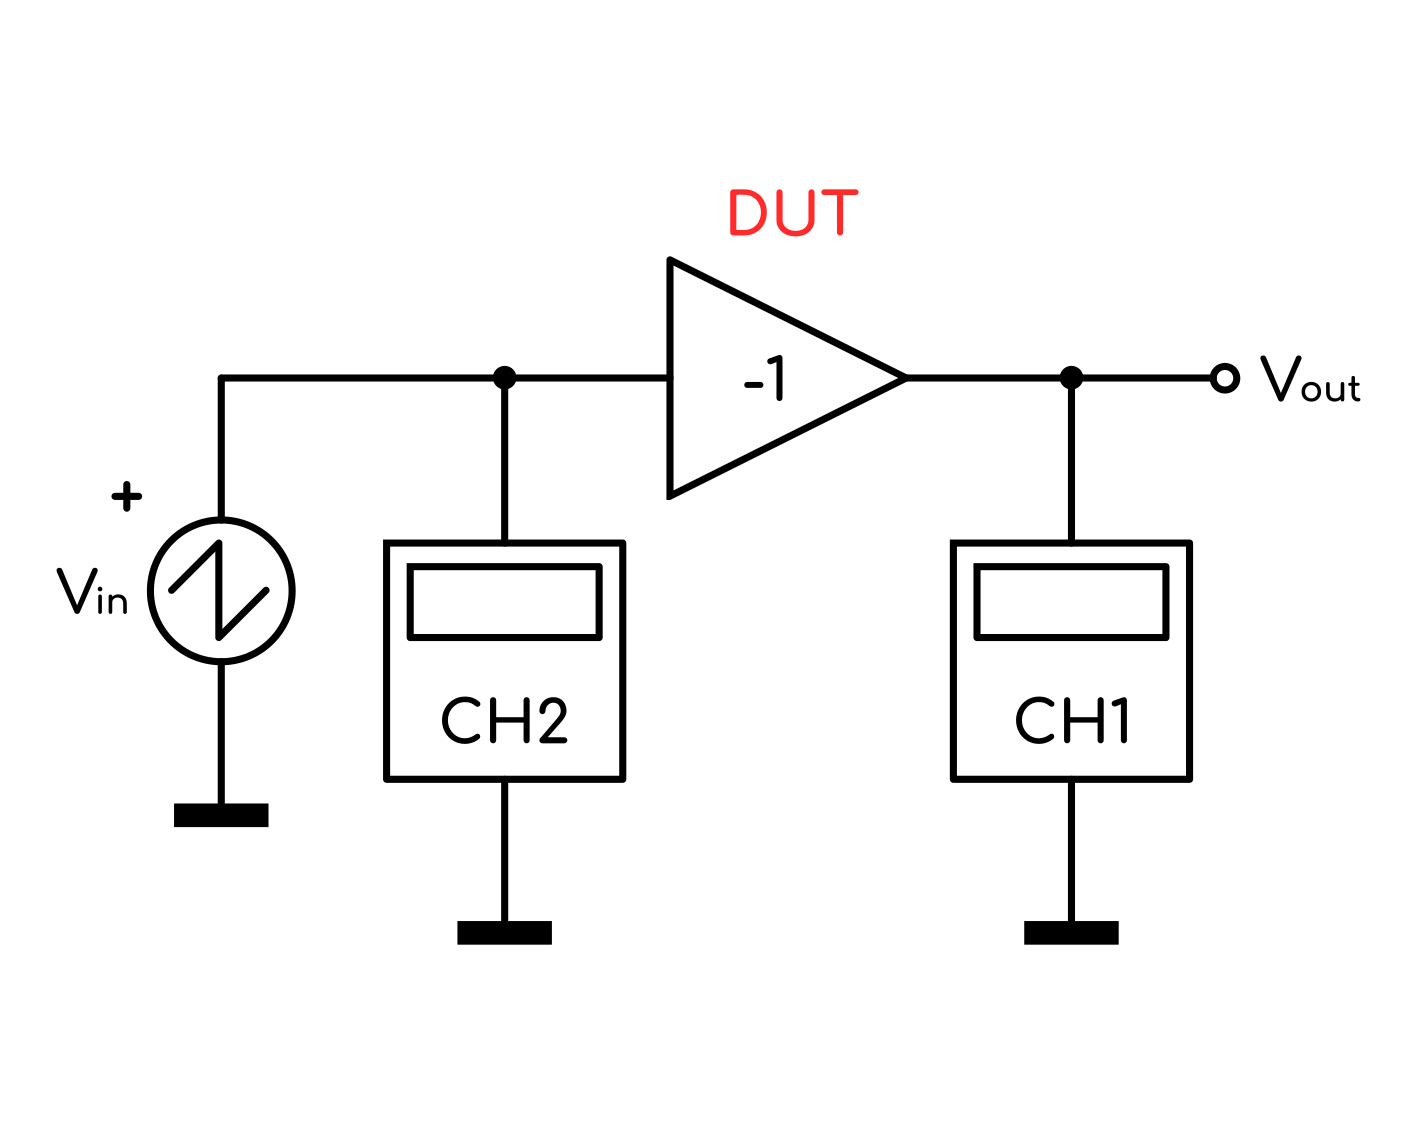
\includegraphics{block_diagrams/mis_saw.png}
        \caption{Setup di misura}
        \label{mis_saw}
    \end{subfigure}%
    \begin{subfigure}{.5\textwidth}
        \centering
        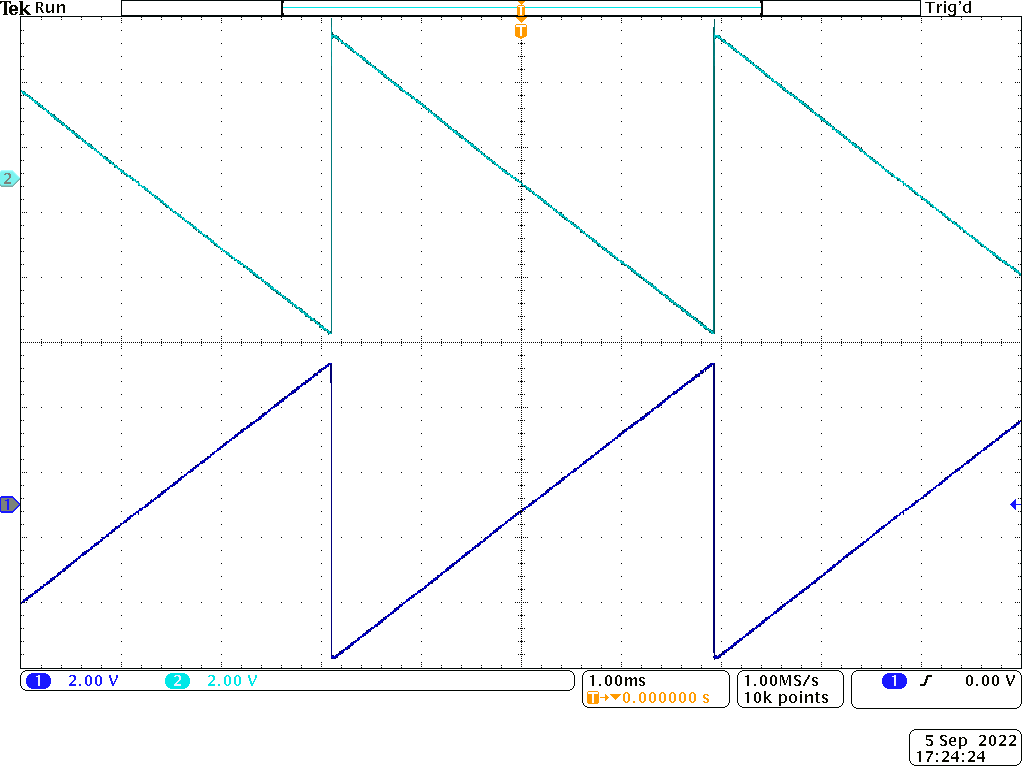
\includegraphics[scale = 0.2]{acquisitions/saw_wave.png}
        \caption{Acquisizione dell'onda ottenuta}
        \label{acq_saw}
    \end{subfigure}

    \caption{Misura del segnale a dente di sega}
\end{figure}

%--------------------------------------------------------------------------------------------

\section{Onda Quadra}

%--------------------------------------------------------------------------------------------

Anche l'onda quadra risulta piuttosto semplice da generare, in quanto è necessario solo
aggiungere un offset e un guadagno al segnale utilizzato per il pilotaggio del contatore
bidirezionale, ovvero $U/D$. Tale segnale infatti ha già forma e frequenza desiderate, è però
compresa solo tra $0\ V$ e $+5\ V$, e si deve estendere fino a $-5\ V$.
Si utilizza quindi un altro amplificatore invertente con uno schema leggermente diverso dai
precedenti:

\begin{figure}[H]
    \centering
    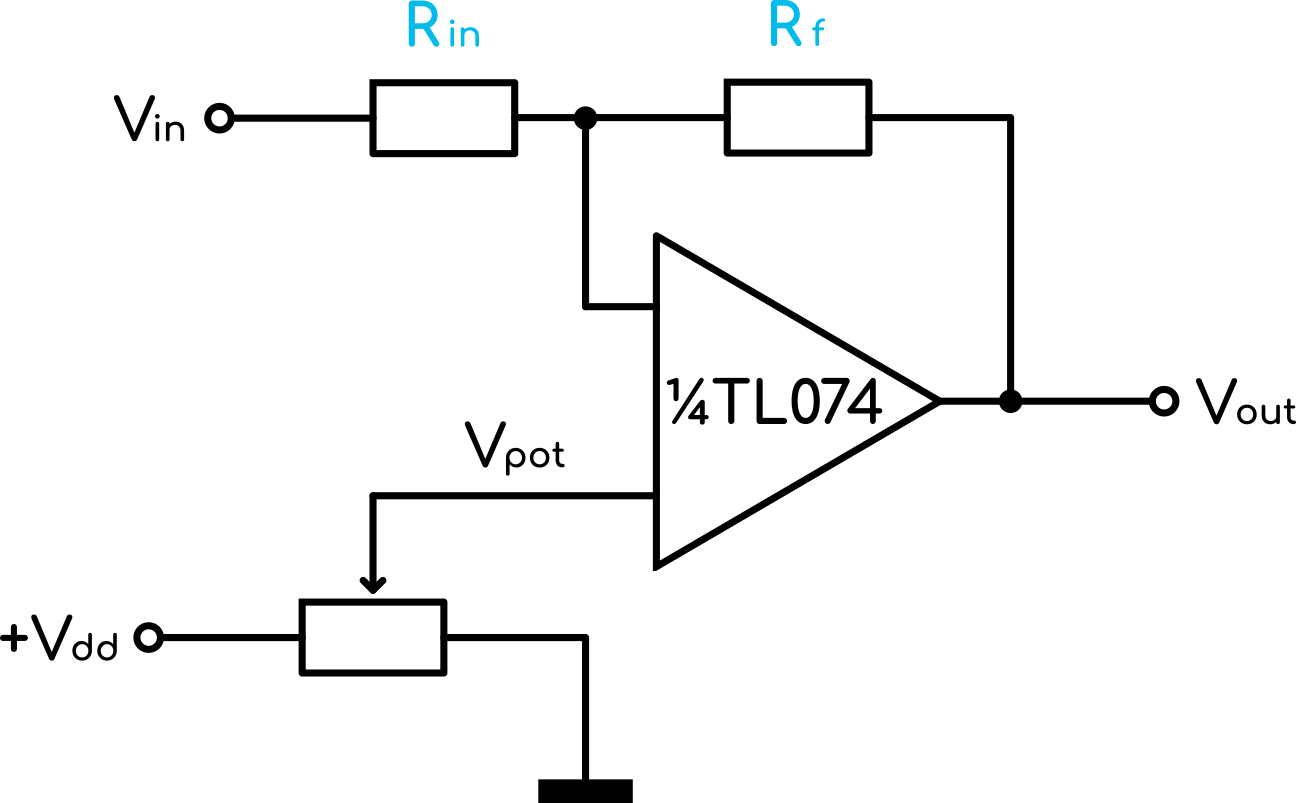
\includegraphics{circuits/inverting_amp_offset_circuit.png}
    \caption{Schema dell'amplificatore invertente con offset ($+V_{dd}=+5\ V$)}
    \label{inverting_amp_offset_circuit}
\end{figure}

in cui si utilizzano due trimmer per la regolazione precisa di guadagno e offset.

La relazione ingresso/uscita è:

\begin{equation}
    V_{out}=V_{pot}\left(1+\frac{R_f}{R_{in}}\right)-V_{in}\frac{R_f}{R_{in}}\ [V]
\end{equation}

dove si vede chiaramente che $-\frac{R_f}{R_{in}}$ è il guadagno e $V_{pot}\left(1+\frac{R_f}{R_{in}}\right)$
l'offset.

La forma d'onda osservata in uscita è quindi la seguente:

\begin{figure}[H]
    \centering

    \begin{subfigure}{.5\textwidth}
        \centering
        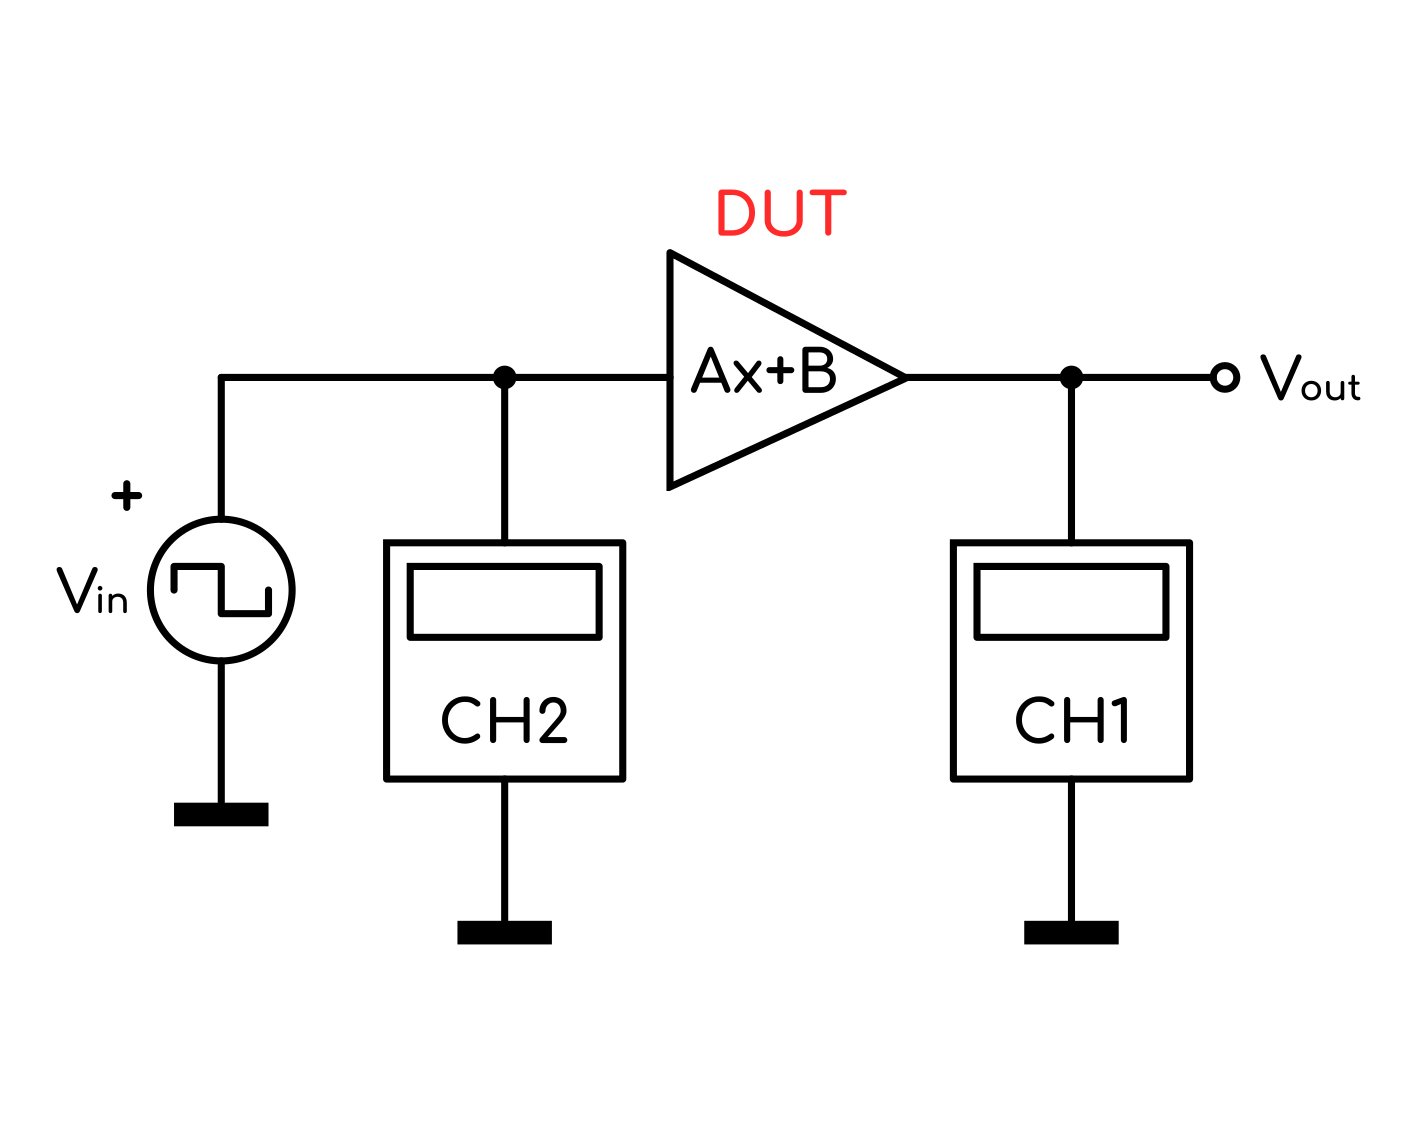
\includegraphics{block_diagrams/mis_square.png}
        \caption{Setup di misura}
        \label{mis_square}
    \end{subfigure}%
    \begin{subfigure}{.5\textwidth}
        \centering
        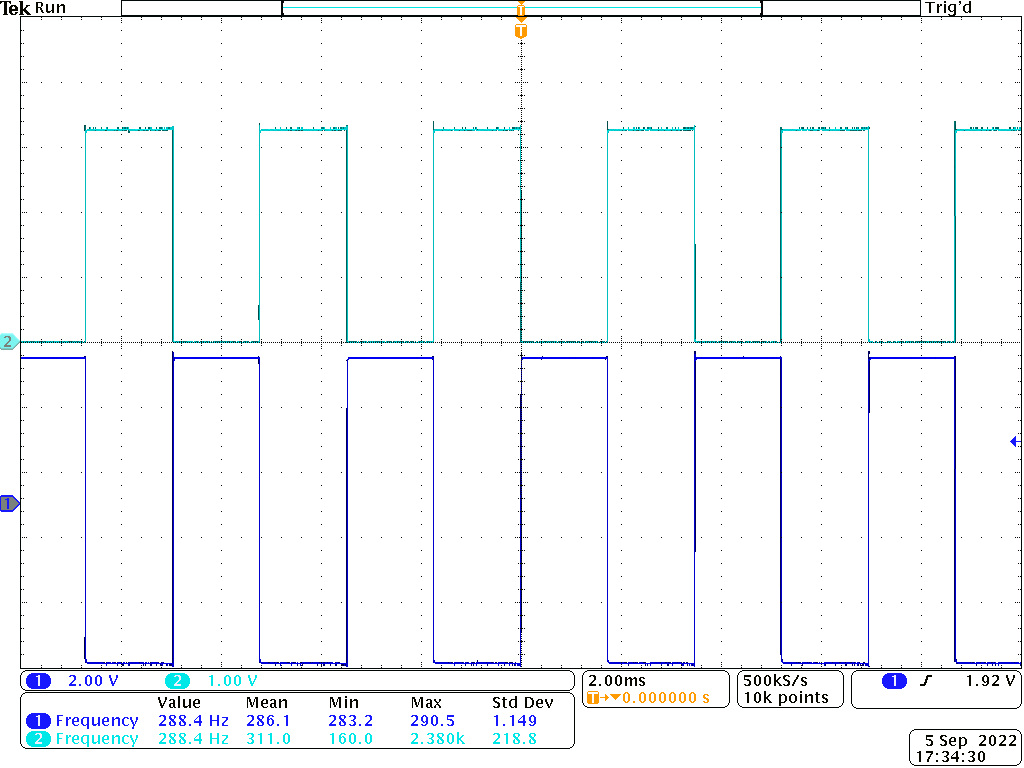
\includegraphics[scale = 0.2]{acquisitions/square_wave.png}
        \caption{Acquisizione dell'onda ottenuta}
        \label{acq_square}
    \end{subfigure}

    \caption{Misura del segnale a onda quadra ottenuto}
\end{figure}

%--------------------------------------------------------------------------------------------

\section{Impulso}

%--------------------------------------------------------------------------------------------

Per quanto riguarda l'impulso invece, facciamo uso del segnale $RCO$ ricavato al capitolo
\ref{segnali_principali}, figura \ref{ramp_counter_circuit}. Tale segnale viene portato in
ingresso ad un circuito monostabile realizzato con il celebre NE555 \cite{ne555} che si
occuperà di invertire la logica dell'impulso. Lo schema utilizzato, è riportato in figura
\ref{monostable_circuit} e viene preso da pg.10 del datasheet.

\begin{figure}[H]
    \centering
    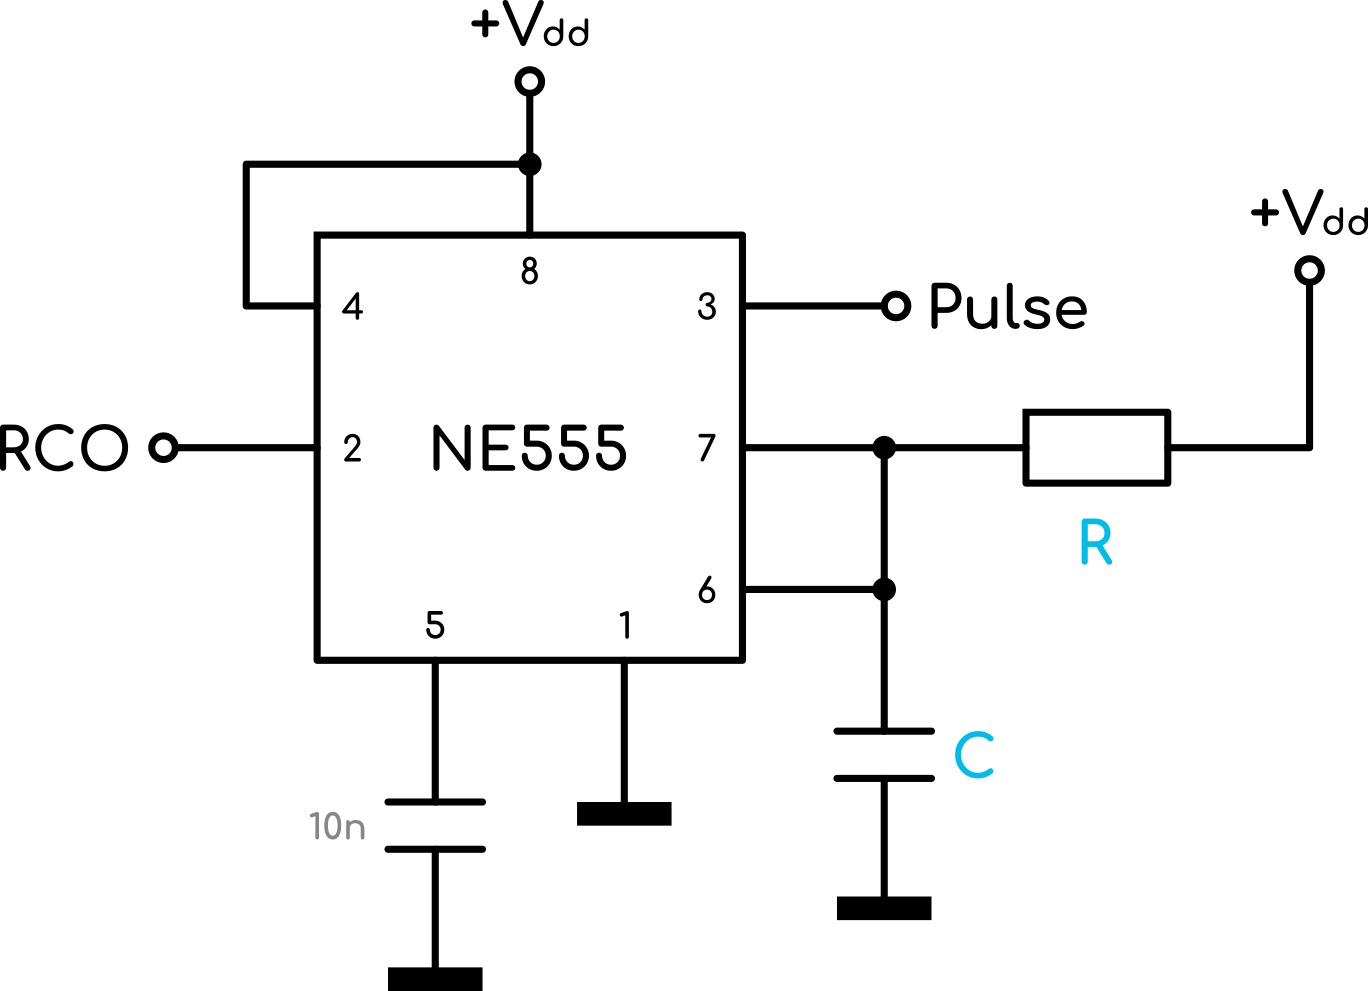
\includegraphics{circuits/monostable_circuit.png}
    \caption{Schema circuito monostabile ($+V_{dd}=+5\ V$)}
    \label{monostable_circuit}
\end{figure}

Si scelgono $R=10\ k\Omega$ e $C=100\ pF$ e si osservano quindi le forme d'onda così ottenute:

\begin{figure}[H]
    \centering
    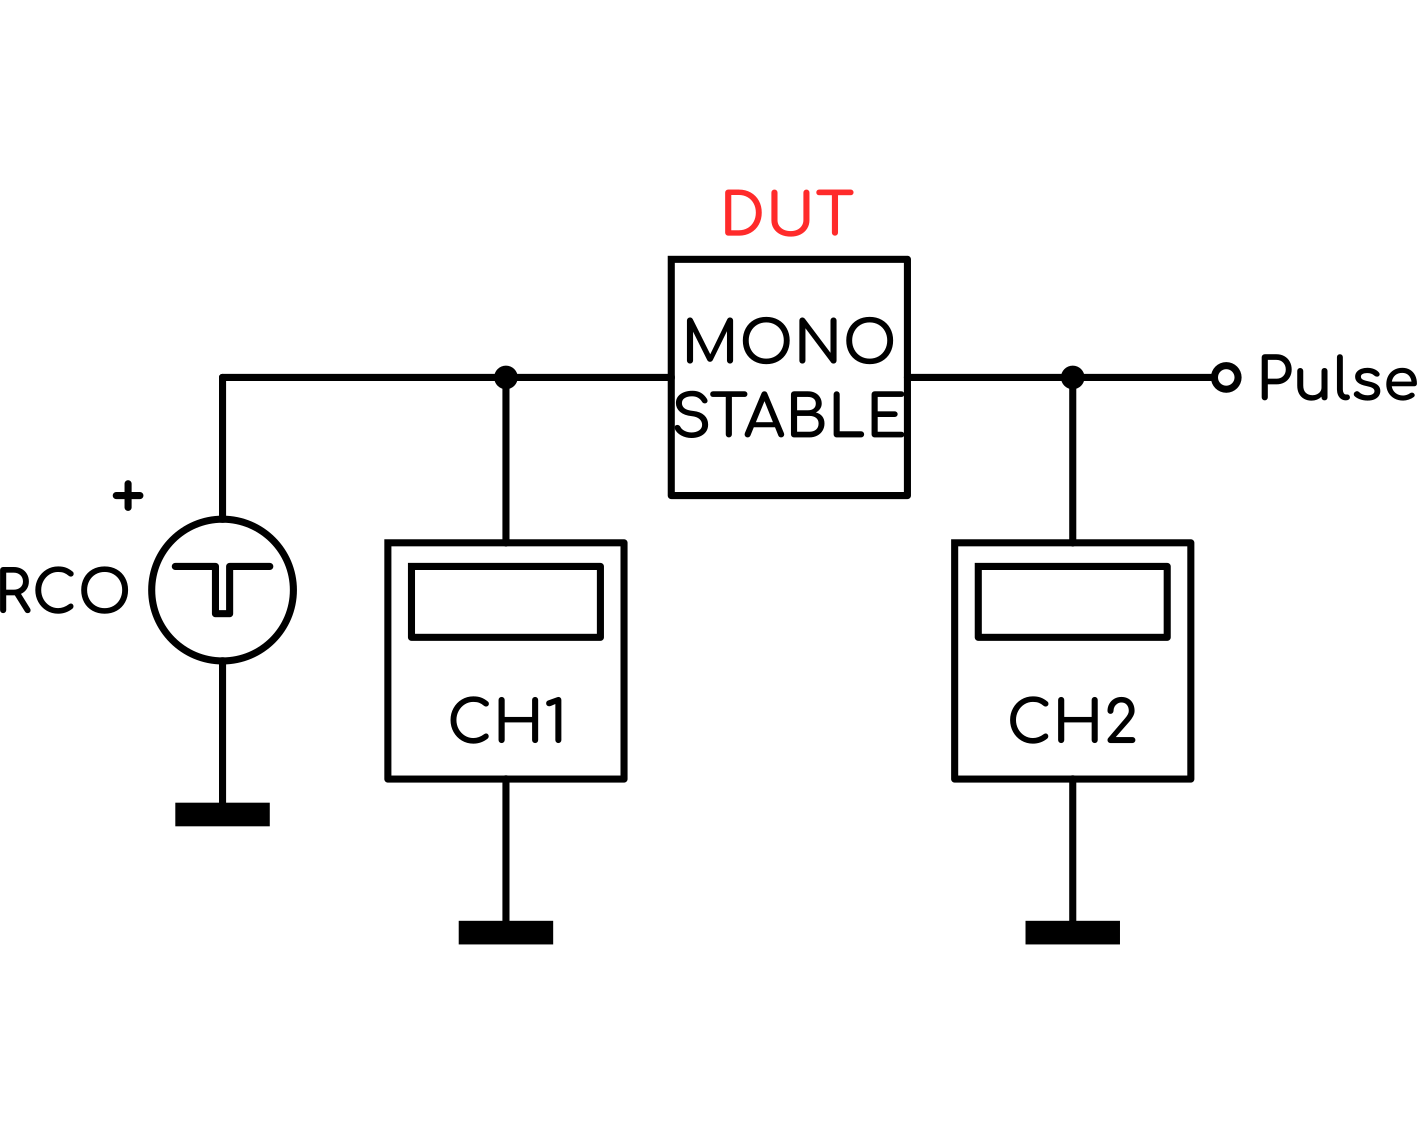
\includegraphics{block_diagrams/mis_monostable.png}
    \caption{Setup di misura del circuito monostabile}
    \label{mis_monostable}
\end{figure}

\begin{figure}[H]
    \centering

    \begin{subfigure}{.5\textwidth}
        \centering
        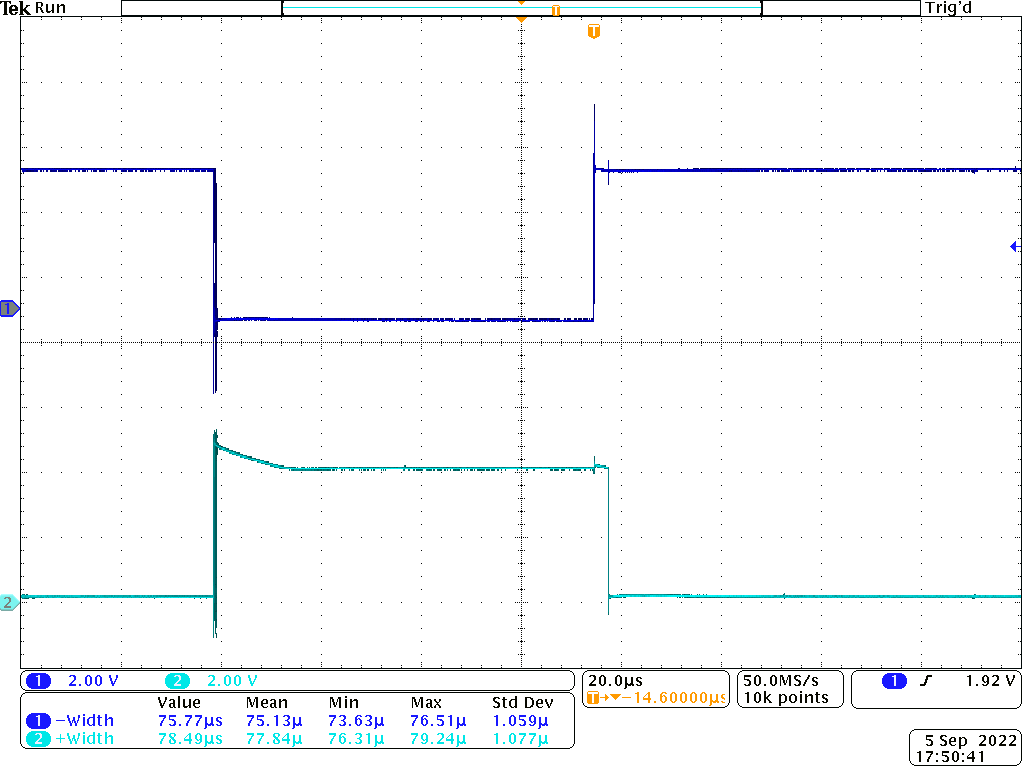
\includegraphics[scale = 0.2]{acquisitions/pulse_2V.png}
        \caption{$V_{in}=+2\ V$}
        \label{acq_monostable_2V}
    \end{subfigure}%
    \begin{subfigure}{.5\textwidth}
        \centering
        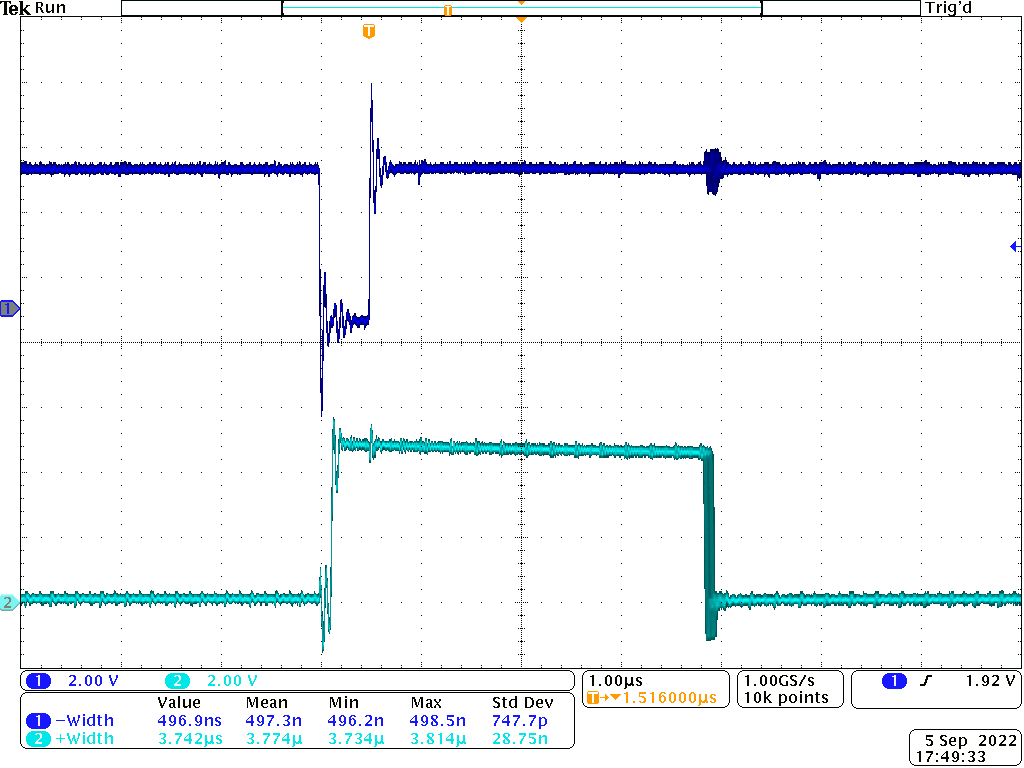
\includegraphics[scale = 0.2]{acquisitions/pulse_8V.png}
        \caption{$V_{in}=+8\ V$}
        \label{acq_monostable_8V}
    \end{subfigure}

    \caption{Acquisizioni dei segnali $RCO$ e $Pulse$ per diversi valori di $V_{in}$}
    \label{mis_pulse}
\end{figure}

%--------------------------------------------------------------------------------------------

\section{Sinusoide}

%--------------------------------------------------------------------------------------------

Infine, l'onda più complicata da generare, ma più semplice dal punto di vista musicale è la
sinusoide. Un metodo piuttosto rapido per generarla consisterebbe nel filtrare al massimo una
qualsiasi delle onde già generate, e lasciare solo l'armonica fondamentale. Tuttavia questo
metodo risulta scomodo se la frequenza del segnale varia in un ampio intervallo di valori,
proprio come nel nostro caso, perchè per ottenere un risultato ottimale la frequenza di taglio
del filtro dovrebbe seguire di pari passo quella dell'oscillatore .

La soluzione utilizzata quindi è un circuito con guadagno variabile in base al livello di
tensione del segnale fornito in ingresso, che si occuperà di convertire un'onda triangolare
nella sinusoide voluta. Viene realizzato con un operazionale e dei diodi, sia normali che di
tipo zener, i quali si occupano di modificare la resistenza di feedback e quindi il valore di
guadagno dell'amplificatore nei diversi intervalli di tensione.

\begin{figure}[H]
    \centering
    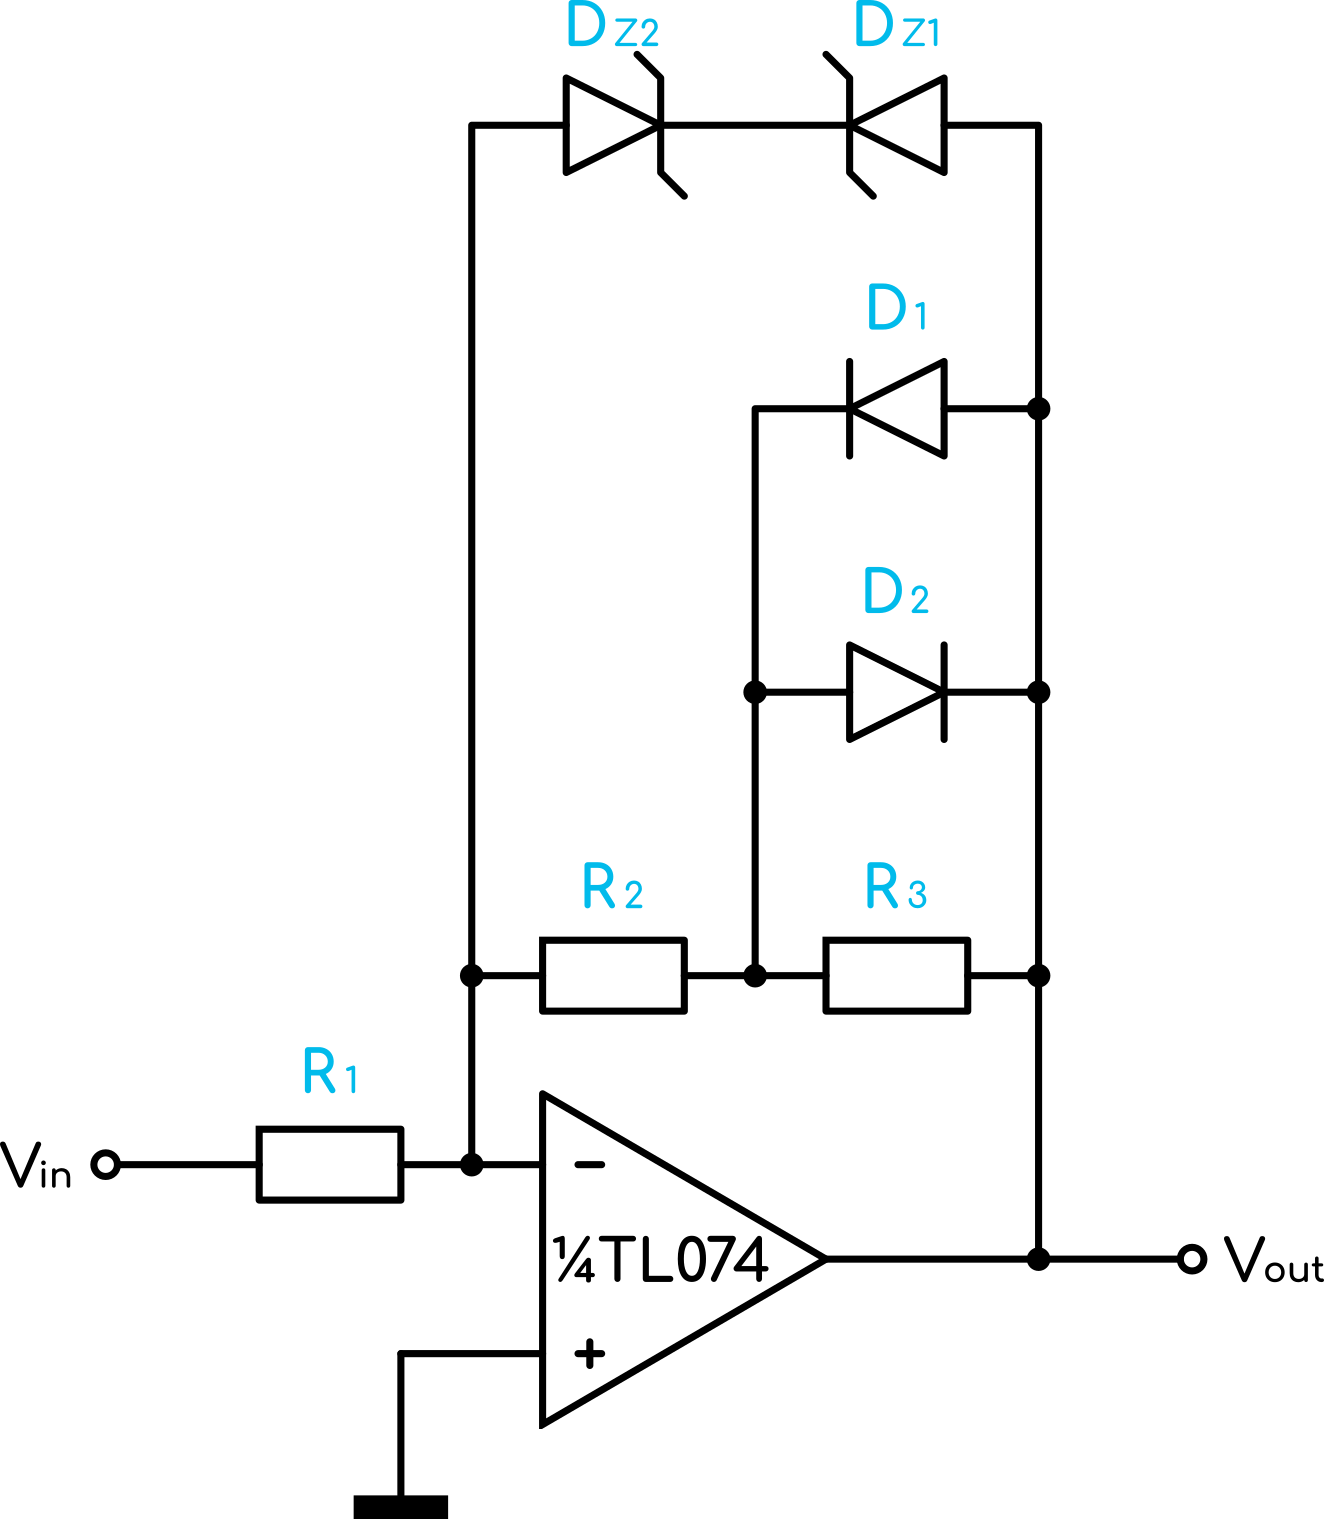
\includegraphics{circuits/sin_circuit.png}
    \caption{Circuito utilizzato per convertire un segnale a triangolo in una sinusoide}
    \label{sin_circuit}
\end{figure}

Per ricavare la relazione ingresso uscita cominciamo con l'osservare che il circuito è
simmetrico rispetto agli $0\ V$, e quindi possiamo limitare l'analisi ai soli valori positivi
di $V_s$ ed estendere poi i risultati al semipiano negativo. Procediamo quindi per casi:

\begin{itemize}
    \item Diodi OFF:

          Tutti i diodi sono interdetti e il circuito equivalente è quello di un amplificatore invertente
          la cui relazione ingresso/uscita è ricavata facilmente.

          \begin{minipage}{0.45\textwidth}
              \centering
              \begin{figure}[H]
                  \centering
                  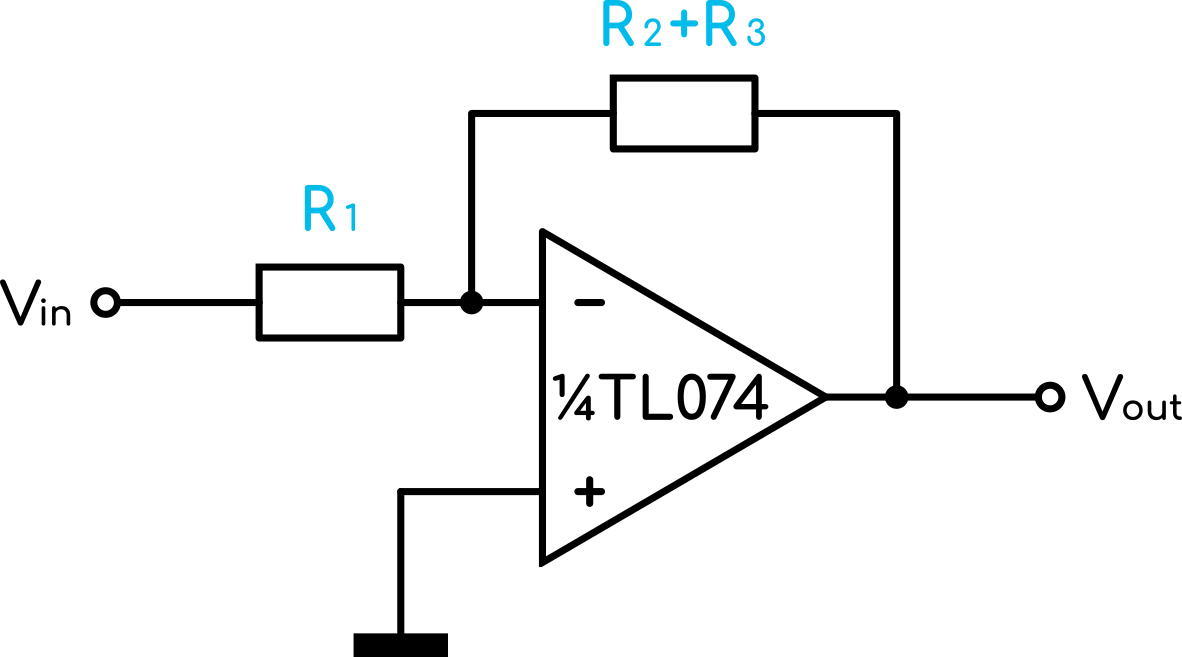
\includegraphics{circuits/sin_case1_circuit.png}
                  \caption{Circuito equivalente}
                  \label{sin_case1_circuit}
              \end{figure}
          \end{minipage}
          \begin{minipage}{0.45\textwidth}
              \centering
              \begin{equation}
                  V_{out}=-V_s\frac{R_2+R_3}{R_1}\ [V]
              \end{equation}
          \end{minipage}

          Questo vale nelle seguenti condizioni:

          \begin{equation}
              \left\{
              \begin{array}{ll}
                  V_{D2}\leq V_{\gamma}        & \rightarrow V_s\leq V_{\gamma}\frac{R_1}{R_3}=V_{TH1}          \\
                  V_{out}\geq-(V_{\gamma}+V_Z) & \rightarrow V_s\leq(V_{\gamma}+V_Z)\frac{R_1}{R_2+R_3}=V_{TH2}
              \end{array}
              \right.
          \end{equation}

    \item $D_2$ ON:

          Solo $D_2$ è attivo e modifica il guadagno del circuito.

          \begin{minipage}{0.45\textwidth}
              \centering
              \begin{figure}[H]
                  \centering
                  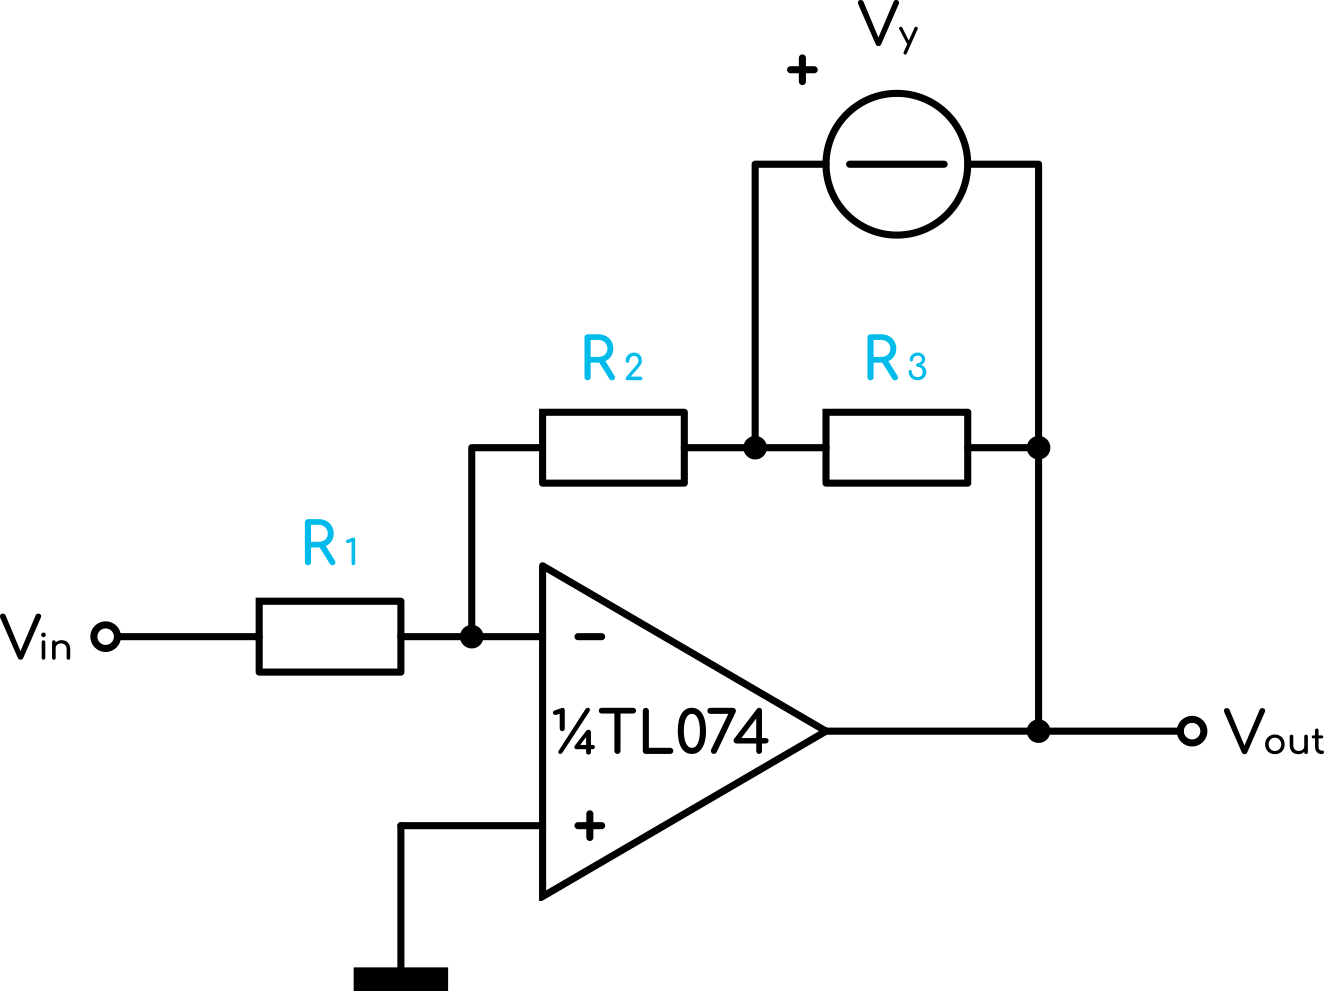
\includegraphics{circuits/sin_case2_circuit.png}
                  \caption{Circuito equivalente}
                  \label{sin_case2_circuit}
              \end{figure}
          \end{minipage}
          \begin{minipage}{0.45\textwidth}
              \centering
              \begin{equation}
                  V_{out}=-V_s\frac{R_2}{R_1}-V_\gamma\ [V]
              \end{equation}
          \end{minipage}

          che ha valore per le seguenti condizioni:

          \begin{equation}
              \left\{
              \begin{array}{ll}
                  I_{D2}> 0                    & \rightarrow V_s>V_{TH1}                        \\
                  V_{out}\geq-(V_{\gamma}+V_Z) & \rightarrow V_s\leq V_Z\frac{R_1}{R_2}=V_{TH3}
              \end{array}
              \right.
          \end{equation}

    \item $D_{Z1}$ in scarica, $D_2$ e $D_{Z2}$ ON:

          Infine nell'ultimo caso, l'uscita è determinata dalle cadute di tensione sui diodi.

          \begin{minipage}{0.45\textwidth}
              \centering
              \begin{figure}[H]
                  \centering
                  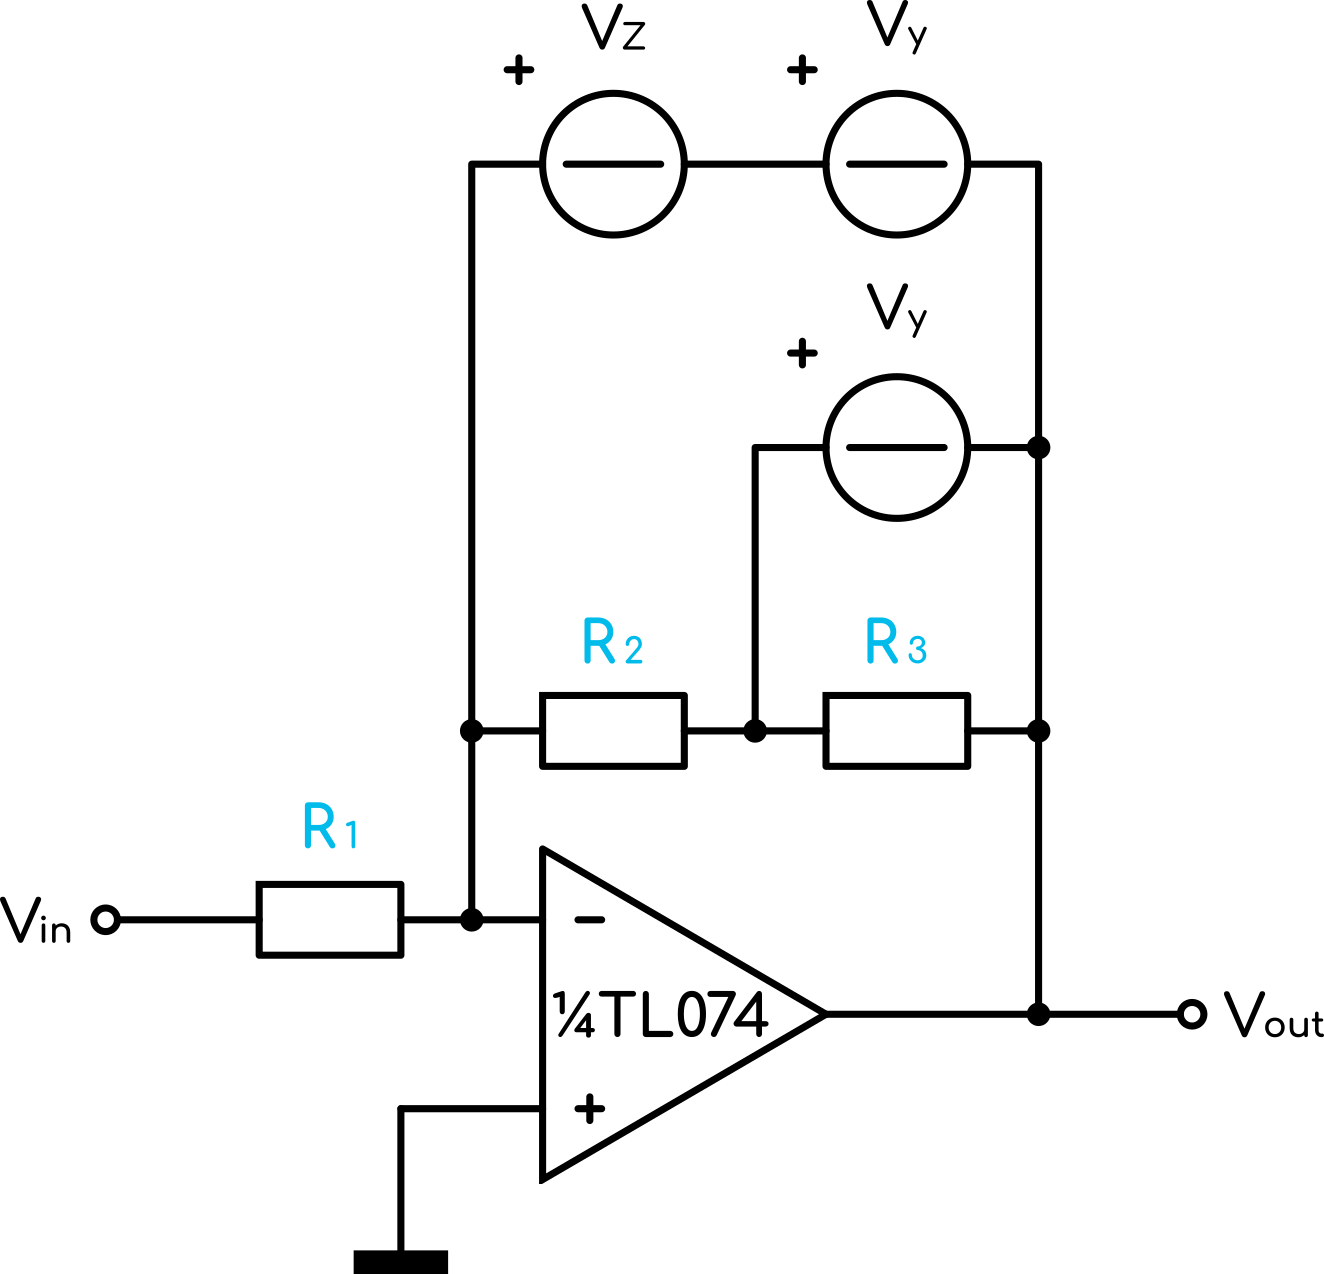
\includegraphics{circuits/sin_case3_circuit.png}
                  \caption{Circuito equivalente}
                  \label{sin_case3_circuit}
              \end{figure}
          \end{minipage}
          \begin{minipage}{0.45\textwidth}
              \centering
              \begin{equation}
                  V_{out}=-(V_{\gamma}+V_Z)\ [V]
              \end{equation}
          \end{minipage}

          Ci troviamo quindi nelle seguenti condizioni:

          \begin{equation}
              \left\{
              \begin{array}{ll}
                  I_{D2}> 0  & \rightarrow V_Z>V_\gamma\frac{R_2}{R_3} \\
                  I_{DZ2}> 0 & \rightarrow V_s>V_{TH3}
              \end{array}
              \right.
          \end{equation}

\end{itemize}

Si utilizzano dei diodi zener con tensione di scarica pari a $3.3\ V$, poichè il segnale in
ingresso è limitato a $+5\ V$, poi procediamo con i valori dei resistori.

Per il primo caso impostiamo guadagno pressochè unitario, quindi otteniamo il vincolo
$R_1\approx R_2+R_3$. Possiamo scegliere $R_1=33\ k\Omega$, $R_2=22\ k\Omega$ e $R_3=12\ k\Omega$.
Questo ci permette di definire i valori di soglia del primo intervallo $V_{TH1}\approx1.93\ V$
e $V_{TH2}\approx3.88\ V$. L'intervallo di funzionamento nella prima configurazione è quindi
$|V_s|\leq V_{TH1}$ visto che $V_{TH2}>V_{TH1}$.

Nel secondo caso invece, il valore di soglia vale $V_{TH3}=4.95\ V$, quindi l'intervallo di
funzionamento è $V_{TH1}<|V_s|\leq V_{TH3}$, e il valore del guadagno risulta
$\frac{R_2}{R_1}\approx0.67$.

Nell'ultimo caso infine, essendo l'uscita completamente determinata dalle cadute di tensione
sui diodi, l'intervallo di funzionamento in questa configurazione è $|V_s|>V_{TH3}$, e
l'uscita viene tagliata a $\approx4\ V$.

\begin{figure}[H]
    \centering
    \begin{tikzpicture}
        \centering
        \begin{axis}[
                title = Transcaratteristica teorica,
                no marks,
                domain = -6:6,
                samples = 100,
                xmin = -6.5, xmax = 6.5,
                ymin = -6.5, ymax = 6.5,
                grid = major,
                grid style = {dashed, gray!30},
                xlabel = $V_{in}$,
                ylabel = $V_{out}$,
                x unit = \si{\V}, y unit = \si{\V},
                legend style = {at = {(0.5, -0.25)}, anchor = north},
                cycle list name = modular,
            ]

            \addplot[
                domain = -1.925:1.925,
                samples = 20,
                color = myBlue,
            ]{-34*x/33};

            \addplot[
                domain = 1.925:4.95,
                samples = 20,
                color = myBlue,
            ]{-22*x/33-0.7};

            \addplot[
                domain = -4.95:-1.925,
                samples = 20,
                color = myBlue,
            ]{-22*x/33+0.7};

            \addplot[
                domain = 4.95:6,
                samples = 20,
                color = myBlue,
            ]{-4};

            \addplot[
                domain = -6:-4.95,
                samples = 20,
                color = myBlue,
            ]{4};
        \end{axis}
    \end{tikzpicture}
\end{figure}

Poichè in questo passaggio la tensione massima ottenuta è limitata a $4\ V$ (a causa dei diodi),
è anche necessario uno stadio amplificatore in cascata per riportare l'onda ai livelli di
tensione specificati dallo standard.

\begin{figure}[H]
    \centering
    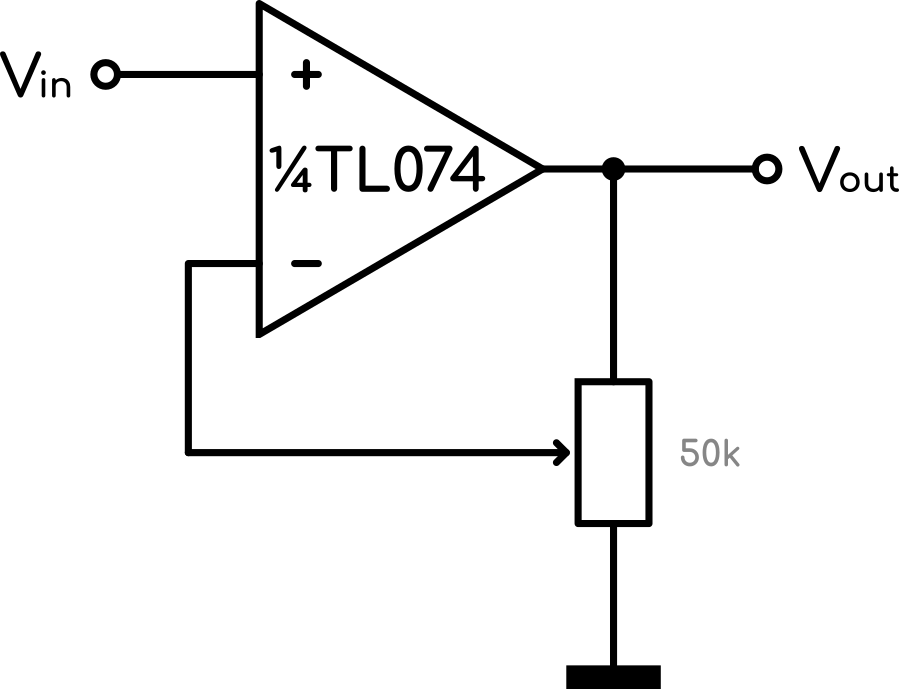
\includegraphics{circuits/noninverting_amp_circuit.png}
    \caption{Amplificatore non-invertente}
    \label{noninverting_amp_circuit}
\end{figure}

Osserviamo quindi l'onda ottenuta e verifichiamo quanto risulta buona come approssimazione:

\begin{figure}[H]
    \centering
    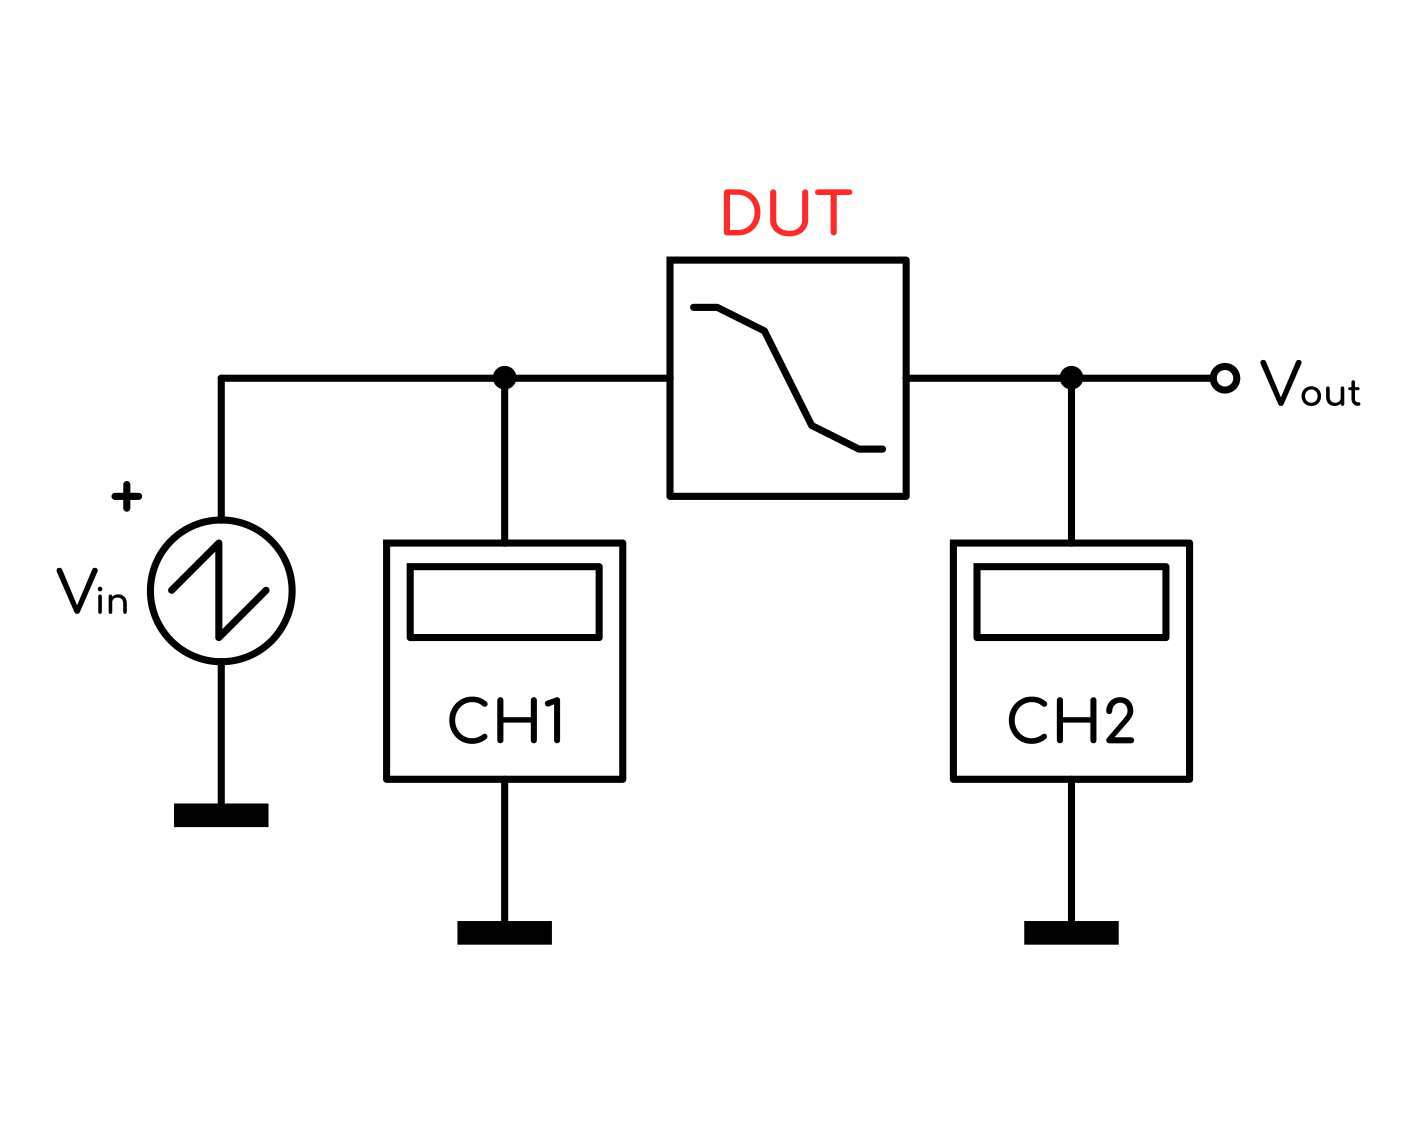
\includegraphics{block_diagrams/mis_sin_oscilloscope.png}
    \caption{Setup di misura}
    \label{mis_sin_oscilloscope}
\end{figure}

\begin{figure}[H]
    \centering

    \begin{subfigure}{.5\textwidth}
        \centering
        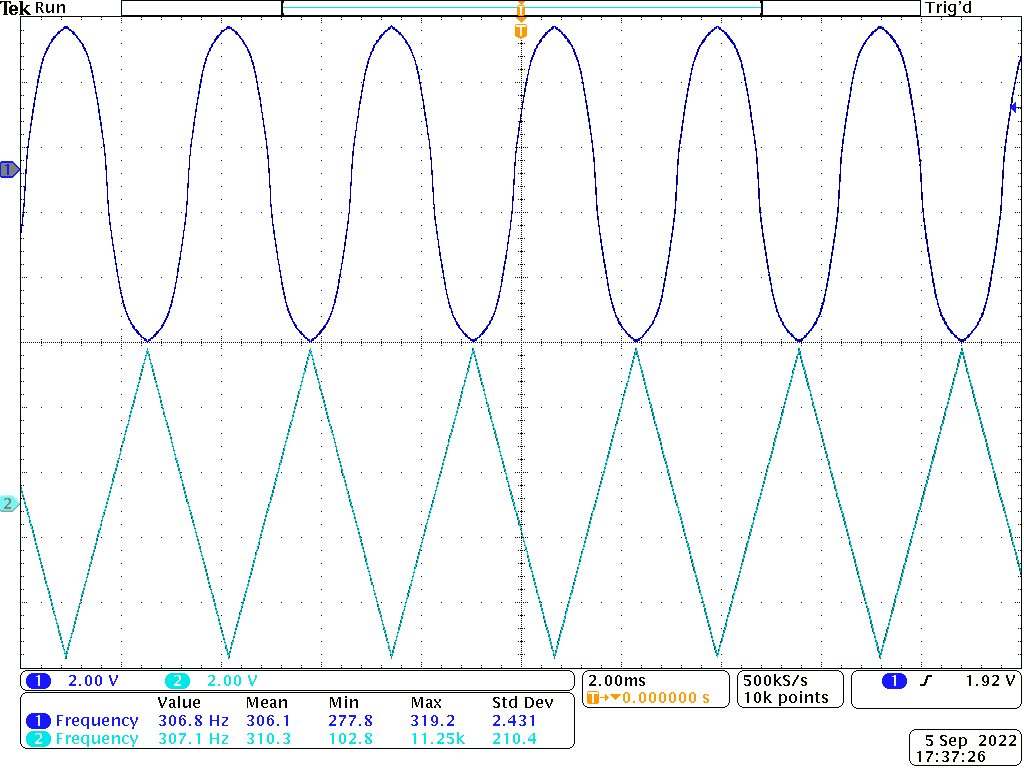
\includegraphics[scale = 0.2]{acquisitions/sine_wave_2V.png}
        \caption{$V_{in}=+2\ V$}
        \label{acq_sine_2V}
    \end{subfigure}%
    \begin{subfigure}{.5\textwidth}
        \centering
        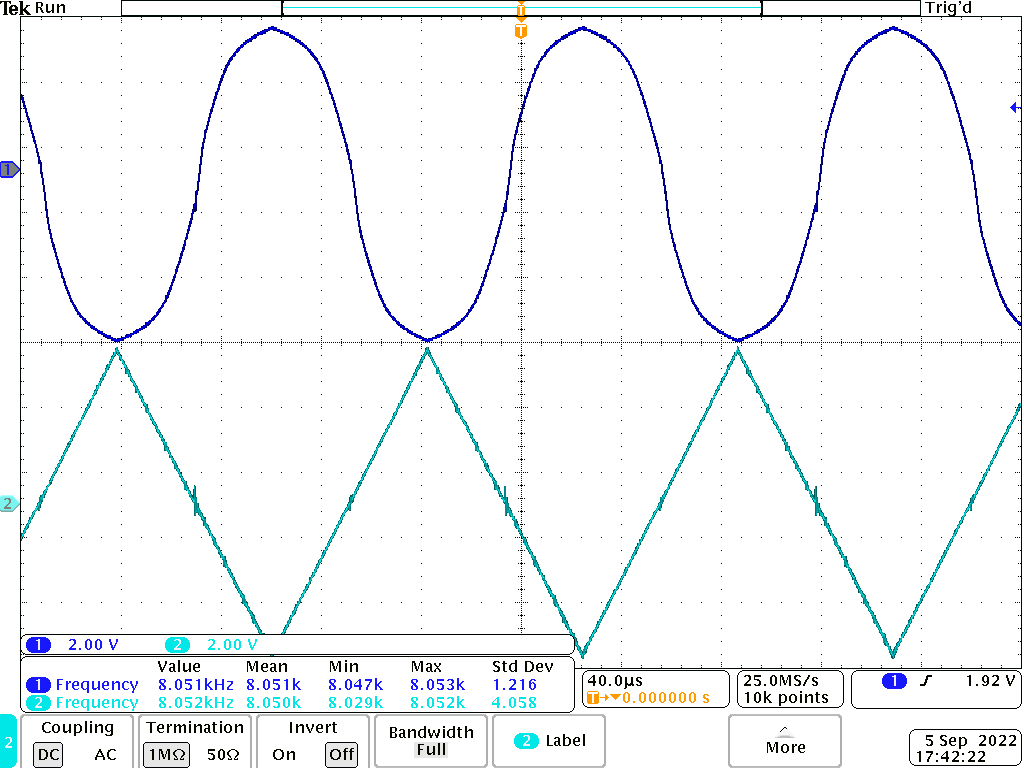
\includegraphics[scale = 0.2]{acquisitions/sine_wave_8V.png}
        \caption{$V_{in}=+8\ V$}
        \label{acq_sine_8V}
    \end{subfigure}
    \begin{subfigure}{.5\textwidth}
        \centering
        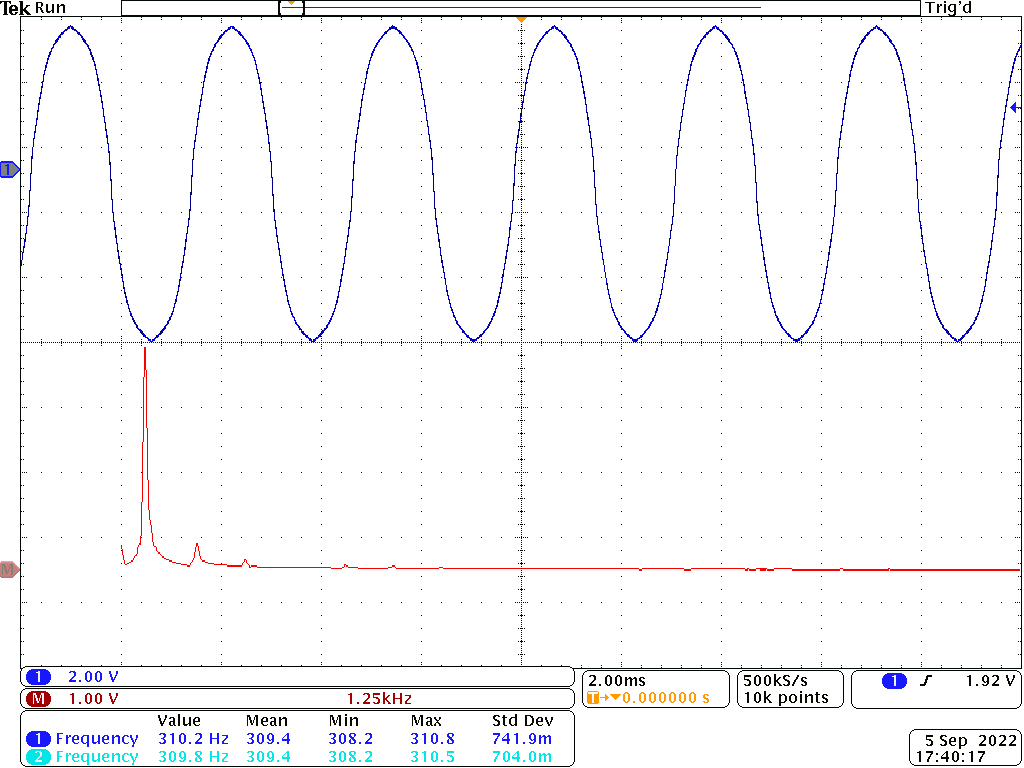
\includegraphics[scale = 0.2]{acquisitions/sine_spectrum_2V.png}
        \caption{$V_{in}=+2\ V$}
        \label{acq_fourier_2V}
    \end{subfigure}%
    \begin{subfigure}{.5\textwidth}
        \centering
        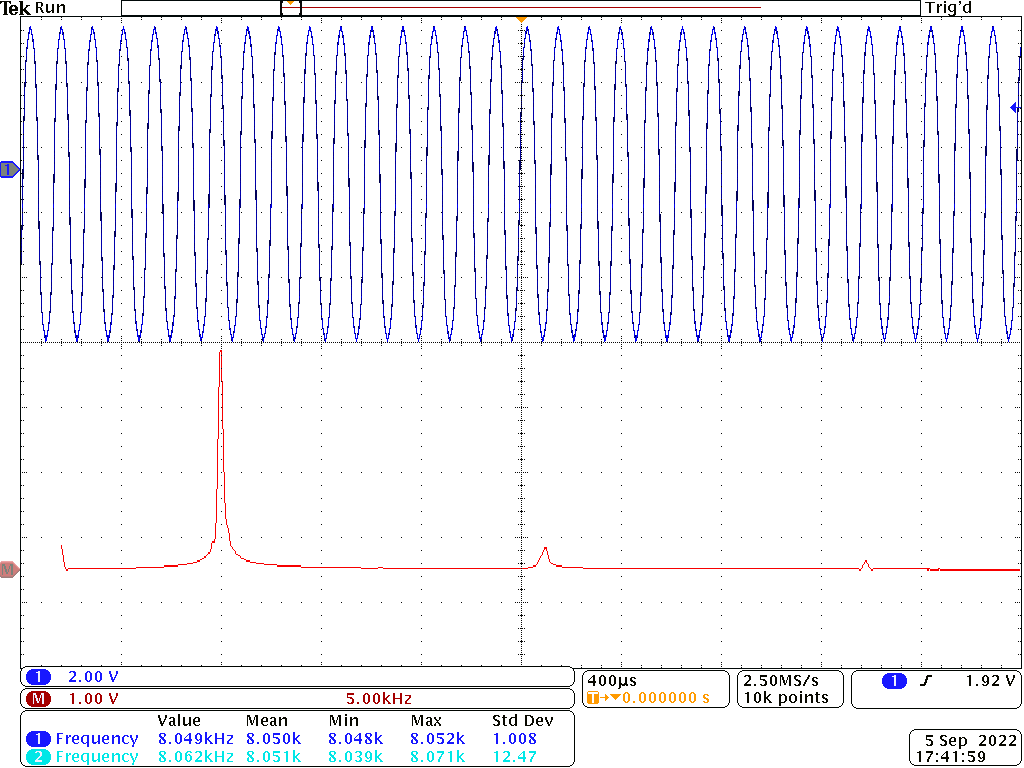
\includegraphics[scale = 0.2]{acquisitions/sine_spectrum_8V.png}
        \caption{$V_{in}=+8\ V$}
        \label{acq_fourier_8V}
    \end{subfigure}

    \caption{Sinusoide ottenuta per diversi valori di $V_{in}$ nel dominio del tempo e
        della frequenza}
    \label{acq_sine}
\end{figure}

Dall'analisi in frequenza vediamo che le armoniche del rumore sono pressochè ininfluenti e
quindi l'onda ottenuta risulta effettivamente un'ottima approssimazione di una sinusoide.
Sl variare della frequenza poi, la bontà dell'onda non cambia, come invece sarebbe successo
se avessimo impiegato un filtro.

\begin{figure}[H]
    \centering
    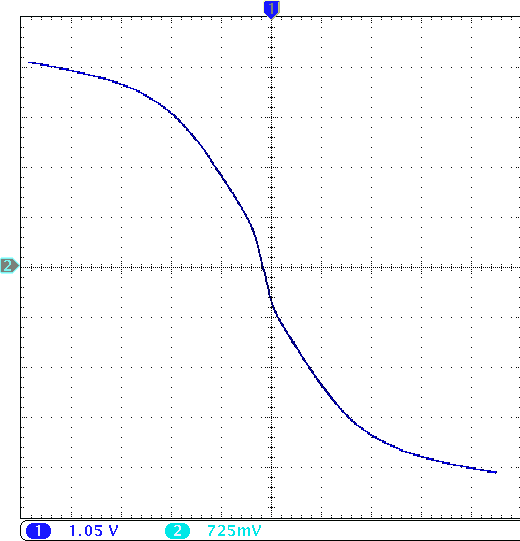
\includegraphics[scale = 0.5]{acquisitions/trans_sine_cut.png}
    \caption{Transcaratteristica tracciata con l'oscilloscopio}
    \label{acq_sine_oscilloscope}
\end{figure}

Infine, la transcaratteristica tracciata tramite oscilloscopio risulta abbastanza simile a
quella teorica in figura, anche se più smussata a causa del comportamento reale dei diodi.

%--------------------------------------------------------------------------------------------
